\documentclass[12pt,a4paper]{article}

% ─── Page Layout ───────────────────────────────────────────────────────────────
\usepackage[a4paper, margin=0.8in, headheight=14pt]{geometry}

% ─── Fonts (XeLaTeX) ───────────────────────────────────────────────────────────
\usepackage{fontspec}
\usepackage{unicode-math}
\setmainfont{TeX Gyre Pagella}
\setmonofont[Scale=0.88]{TeX Gyre Cursor}
\setmathfont{Latin Modern Math}

% ─── Packages ──────────────────────────────────────────────────────────────────
\usepackage{xcolor}
\usepackage{colortbl}
\usepackage{titlesec}
\usepackage{enumitem}
\usepackage{tabularx}
\usepackage{booktabs}
\usepackage{array}
\usepackage{amsmath}
\usepackage{tikz}
\usetikzlibrary{shapes.geometric, arrows.meta, positioning, calc, fit, decorations.pathreplacing, patterns}
\usepackage{tcolorbox}
\tcbuselibrary{skins, breakable}
\usepackage{hyperref}
\usepackage{fancyhdr}
\usepackage{graphicx}
\usepackage{microtype}
\hyphenpenalty=10000
\exhyphenpenalty=10000
\sloppy
\usepackage{caption}
\usepackage{setspace}
\usepackage{multirow}
\usepackage{tocloft}

% ─── Q&A helper ────────────────────────────────────────────────────────────────
\newcommand{\Q}[1]{\textbf{#1}\par\noindent\ignorespaces}

% ─── Colour Palette ────────────────────────────────────────────────────────────
\definecolor{myred}{RGB}{196,30,58}
\definecolor{mydark}{RGB}{30,30,50}
\definecolor{mygreen}{RGB}{14,120,80}
\definecolor{myteal}{RGB}{0,130,140}
\definecolor{myamber}{RGB}{180,100,0}
\definecolor{mypurple}{RGB}{100,30,160}
\definecolor{mygray}{RGB}{246,247,249}
\definecolor{mgframe}{RGB}{180,185,200}
\definecolor{watermark}{RGB}{145,150,170}
\definecolor{hdrred}{RGB}{250,232,235}
\definecolor{hdrgreen}{RGB}{220,244,233}
\definecolor{hdrteal}{RGB}{220,242,244}
\definecolor{hdramber}{RGB}{253,242,215}
\definecolor{hdrpurple}{RGB}{238,228,255}
\definecolor{hdrgray}{RGB}{238,240,245}
\definecolor{rowalt}{RGB}{250,251,253}

% ─── Section Formatting ────────────────────────────────────────────────────────
\titleformat{\section}
  {\large\bfseries\color{myred}}{\thesection.}{0.5em}{}
  [\vspace{1pt}{\color{myred}\rule{\linewidth}{0.8pt}}]
\titleformat{\subsection}
  {\normalsize\bfseries\color{myteal}}{\thesubsection}{0.5em}{}
\titlespacing*{\section}{0pt}{18pt}{7pt}
\titlespacing*{\subsection}{0pt}{11pt}{4pt}

% ─── Paragraph ─────────────────────────────────────────────────────────────────
\setlength{\parindent}{0pt}
\setlength{\parskip}{4pt}

% ─── TOC Styling ───────────────────────────────────────────────────────────────
\renewcommand{\cfttoctitlefont}{\large\bfseries\color{myred}}
\renewcommand{\cftaftertoctitle}{\par\noindent{\color{myred}\rule{\linewidth}{0.8pt}}}
\setlength{\cftbeforetoctitleskip}{0pt}
\setlength{\cftaftertoctitleskip}{6pt}
\renewcommand{\cftsecfont}{\normalsize\bfseries\color{mydark}}
\renewcommand{\cftsecpagefont}{\normalsize\bfseries\color{mydark}}
\renewcommand{\cftsecleader}{\cftdotfill{\cftdotsep}}
\setlength{\cftbeforesecskip}{7pt}
\renewcommand{\cftsubsecfont}{\small\color{mydark}}
\renewcommand{\cftsubsecpagefont}{\small\color{mydark}}
\setlength{\cftbeforesubsecskip}{3pt}
\setlength{\cftsubsecindent}{1.4em}

% ─── Table helpers ─────────────────────────────────────────────────────────────
\renewcommand{\arraystretch}{1.45}
\setlength{\tabcolsep}{6pt}
\arrayrulecolor{mydark}
\newcolumntype{B}[1]{>{\small\bfseries\raggedright\arraybackslash}m{#1}}
\newcolumntype{Y}{>{\small\raggedright\arraybackslash}X}
\renewcommand{\tabularxcolumn}[1]{m{#1}}

% ─── Header / Footer ───────────────────────────────────────────────────────────
\pagestyle{fancy}
\fancyhf{}
\fancyhead[L]{\small\color{myred}\textbf{EC304}\;\color{mydark}--- Network Theory}
\fancyhead[R]{\small\color{myteal}\textbf{Module 4 Notes}}
\fancyfoot[C]{\small\color{mydark}\thepage}
\fancyfoot[R]{\small\color{watermark}\textit{\copyright\ Biraj}}
\renewcommand{\headrulewidth}{0.5pt}
\renewcommand{\footrulewidth}{0.3pt}

% ─── Hyperref ──────────────────────────────────────────────────────────────────
\hypersetup{
  colorlinks=true, linkcolor=myteal, urlcolor=myteal,
  pdfauthor={Biraj Sarkar (CGEC)},
  pdftitle={EC304 --- Module 4 Notes: Network Functions, Two-Port Networks, Resonance and Filters}
}

% ─── tcolorbox styles ──────────────────────────────────────────────────────────
\tcbset{
  tikzbox/.style={
    colback=mygray, colframe=mgframe, boxrule=0.6pt, arc=4pt,
    left=8pt, right=8pt, top=6pt, bottom=6pt,
    colbacktitle=mgframe, coltitle=mydark,
    fonttitle=\small\bfseries
  },
  defbox/.style={
    colback=hdrgreen, colframe=mygreen, boxrule=0.8pt, arc=4pt,
    left=9pt, right=9pt, top=6pt, bottom=6pt,
    colbacktitle=mygreen, coltitle=white,
    fonttitle=\small\bfseries
  },
  formulabox/.style={
    colback=hdrteal, colframe=myteal, boxrule=0.8pt, arc=4pt,
    left=9pt, right=9pt, top=7pt, bottom=7pt,
    colbacktitle=myteal, coltitle=white,
    fonttitle=\small\bfseries
  },
  examplebox/.style={
    colback=hdramber, colframe=myamber, boxrule=0.8pt, arc=4pt,
    left=9pt, right=9pt, top=6pt, bottom=6pt,
    colbacktitle=myamber, coltitle=white,
    fonttitle=\small\bfseries
  },
  masonbox/.style={
    colback=hdrpurple, colframe=mypurple, boxrule=0.8pt, arc=4pt,
    left=9pt, right=9pt, top=6pt, bottom=6pt,
    colbacktitle=mypurple, coltitle=white,
    fonttitle=\small\bfseries
  },
  exambox/.style={
    colback=hdrpurple, colframe=mypurple, boxrule=1pt, arc=5pt,
    left=10pt, right=10pt, top=8pt, bottom=8pt,
    colbacktitle=mypurple, coltitle=white,
    fonttitle=\bfseries,
    breakable, title after break={\textbf{Frequently Asked / Viva Questions (contd.)}}
  }
}
\tcbset{breakable}
\tcbset{after={\color{black}}}

% ─── TikZ styles ───────────────────────────────────────────────────────────────
\tikzset{
  circnode/.style={circle, draw=myteal, fill=hdrteal, inner sep=2pt, minimum size=6pt},
  sourcenode/.style={circle, draw=myred, fill=hdrred, minimum size=0.9cm, font=\small\bfseries, align=center},
  depnode/.style={diamond, draw=myred, fill=hdrred, minimum size=1.0cm, font=\small\bfseries, align=center},
  block/.style={rectangle, draw=myteal, fill=hdrteal, text width=2.4cm, align=center, minimum height=0.95cm, font=\small, rounded corners=3pt, line width=0.7pt},
  arrow/.style={-Stealth, thick, color=mydark},
  redarrow/.style={-Stealth, thick, color=myred},
  line/.style={thick, color=mydark}
}

\begin{document}

% ─── Title Block ───────────────────────────────────────────────────────────────
\begin{center}
  {\LARGE\bfseries\color{myred} EC304 --- Network Theory}\\[5pt]
  {\normalsize\color{mydark} Semester III \quad$\bullet$\quad 3L:0T:0P \quad$\bullet$\quad 3 Credits}\\[3pt]
  {\normalsize\color{myteal}\textbf{Module 4 Exam Notes: Network Functions, Two-Port Networks, Resonance \& Filters}}\\[3pt]
  {\small\color{mydark} CGEC \;$|$\; B.Tech ECE (2023--27) \;$|$\; \textit{Biraj Sarkar}}
\end{center}
\vspace{2pt}\noindent{\color{myred}\rule{\linewidth}{1.5pt}}\vspace{2pt}

\hypersetup{linkcolor=mydark}
\tableofcontents
\hypersetup{linkcolor=myteal}
\newpage

% ===============================================================================
% SECTION 1: COMPLEX FREQUENCY AND NETWORK FUNCTIONS
% ===============================================================================
\section{Complex Frequency and Network Functions}

The concept of complex frequency generalizes real sinusoidal and exponential signals into a unified mathematical framework. It forms the foundation for characterizing linear time-invariant (LTI) networks in the complex frequency $s$-plane.

\subsection{Concept of Complex Frequency}

\begin{tcolorbox}[defbox, title={\textbf{Definition of Complex Frequency}}]
A generalized damped sinusoidal signal is expressed as:
\begin{equation}
  f(t) = A\,e^{\sigma t}\,\cos(\omega t + \theta) = \text{Re}\left\{ A\,e^{j\theta}\,e^{(\sigma + j\omega)t} \right\} = \text{Re}\left\{ \mathbf{F}\,e^{st} \right\}
\end{equation}
The parameter $s = \sigma + j\omega$ is the \textbf{complex frequency} (measured in $\text{s}^{-1}$ or complex nepers/radians per second):
\begin{itemize}[leftmargin=*]
  \item $\sigma = \text{Re}(s)$ is the \textbf{Neper frequency} (damping or growth rate in Np/s).
  \item $\omega = \text{Im}(s)$ is the \textbf{radian angular frequency} (oscillation rate in rad/s).
\end{itemize}
\end{tcolorbox}

\begin{tcolorbox}[formulabox, title={\textbf{Special Cases of the Complex Frequency Variable $s = \sigma + j\omega$}}]
\begin{enumerate}[leftmargin=*]
  \item $\sigma = 0, \omega = 0 \implies s = 0$: Constant DC signal ($f(t) = A$).
  \item $\sigma \ne 0, \omega = 0 \implies s = \sigma$: Pure exponential signal ($e^{\sigma t}$; decaying if $\sigma < 0$, growing if $\sigma > 0$).
  \item $\sigma = 0, \omega \ne 0 \implies s = j\omega$: Undamped steady-state sinusoidal signal ($A\cos(\omega t)$).
  \item $\sigma < 0, \omega \ne 0$: Damped sinusoidal signal (exponentially decaying oscillatory transient).
  \item $\sigma > 0, \omega \ne 0$: Growing sinusoidal signal (unstable active system).
\end{enumerate}
\end{tcolorbox}

\subsection{Definition and Classification of Network Functions}

\begin{tcolorbox}[defbox, title={\textbf{Network Function Definition}}]
For a linear, lumped, time-invariant network with all initial conditions set to zero (relaxed state), a \textbf{Network Function} $H(s)$ is defined as the ratio of the Laplace transform of the output response $R(s)$ to the Laplace transform of the input excitation $E(s)$:
\begin{equation}
  H(s) = \frac{R(s)}{E(s)} \iff R(s) = H(s) \cdot E(s)
\end{equation}
\end{tcolorbox}

Network functions are broadly classified into two categories:
\begin{enumerate}[leftmargin=*]
  \item \textbf{Driving-Point Immittance Functions:} Excitation and response are measured at the \textbf{same port}:
  \begin{itemize}
    \item \textit{Driving-point impedance:} $Z_{in}(s) = \dfrac{V_1(s)}{I_1(s)}$
    \item \textit{Driving-point admittance:} $Y_{in}(s) = \dfrac{I_1(s)}{V_1(s)} = \dfrac{1}{Z_{in}(s)}$
  \end{itemize}
  \item \textbf{Transfer Functions:} Excitation and response are measured at \textbf{different ports}:
  \begin{itemize}
    \item \textit{Voltage Transfer Function (Gain):} $G_{21}(s) = \dfrac{V_2(s)}{V_1(s)}$
    \item \textit{Current Transfer Function (Gain):} $\alpha_{21}(s) = \dfrac{I_2(s)}{I_1(s)}$
    \item \textit{Transfer Impedance:} $Z_{21}(s) = \dfrac{V_2(s)}{I_1(s)}$
    \item \textit{Transfer Admittance:} $Y_{21}(s) = \dfrac{I_2(s)}{V_1(s)}$
  \end{itemize}
\end{enumerate}

% ===============================================================================
% SECTION 2: POLES AND ZEROS OF NETWORK FUNCTIONS
% ===============================================================================
\section{Poles and Zeros of Immittance Functions and their Properties}

Any network function of a lumped LTI circuit can be expressed as a rational function of $s$ with real coefficients:
\begin{equation}
  H(s) = \frac{N(s)}{D(s)} = \frac{a_m s^m + a_{m-1} s^{m-1} + \cdots + a_1 s + a_0}{b_n s^n + b_{n-1} s^{n-1} + \cdots + b_1 s + b_0} = K \frac{\prod_{i=1}^m (s - z_i)}{\prod_{k=1}^n (s - p_k)}
\end{equation}

\subsection{Definitions of Poles and Zeros}

\begin{tcolorbox}[defbox, title={\textbf{Poles and Zeros}}]
\begin{itemize}[leftmargin=*]
  \item \textbf{Zeros ($z_i$):} The values of complex frequency $s$ for which $H(s) = 0$ (roots of the numerator $N(s) = 0$). At a transmission zero, the network completely suppresses the input signal.
  \item \textbf{Poles ($p_k$):} The values of complex frequency $s$ for which $H(s) \to \infty$ (roots of the denominator $D(s) = 0$). Poles define the natural frequencies (modes) and determine stability.
  \item \textbf{Critical Frequencies at Infinity:} If $n > m$, $H(s)$ has $(n - m)$ zeros at $s = \infty$. If $m > n$, $H(s)$ has $(m - n)$ poles at $s = \infty$. The total number of zeros equals the total number of poles in the extended complex plane.
\end{itemize}
\end{tcolorbox}

\subsection{Properties of Driving-Point Immittances (Positive Real Functions)}

For any passive, bilateral electrical network without internal active sources, the driving-point immittance $Z(s)$ or $Y(s)$ must be a \textbf{Positive Real (PR) Function} (Brune's condition):
\begin{equation}
  \text{Re}\{Z(s)\} \ge 0 \quad \text{whenever} \quad \text{Re}(s) \ge 0
\end{equation}

\begin{tcolorbox}[formulabox, title={\textbf{Necessary and Sufficient Properties of Passive Immittance Functions}}]
\begin{enumerate}[leftmargin=*]
  \item \textbf{Hurwitz Denominator and Numerator:} All poles and zeros of $Z(s)$ must lie in the left half of the $s$-plane ($\text{Re}(s) \le 0$). They cannot reside in the open right-half plane (RHP).
  \item \textbf{Imaginary Axis Poles and Zeros:} Any poles and zeros located on the $j\omega$-axis must be \textbf{simple} (multiplicity of 1). Multiple poles on the $j\omega$-axis are strictly forbidden because they generate unbounded polynomial-exponential terms ($t\sin\omega t$).
  \item \textbf{Residue Condition:} The residues of $Z(s)$ at simple poles on the $j\omega$-axis must be \textbf{real and strictly positive}.
  \item \textbf{Degree Constraint:} The degrees of the numerator polynomial $N(s)$ and denominator polynomial $D(s)$ can differ at most by $1$: $|m - n| \le 1$.
  \item \textbf{Lowest Degree Constraint:} The lowest power of $s$ in $N(s)$ and $D(s)$ can differ at most by $1$.
  \item \textbf{Foster Alternation Law (LC Immittance):} For purely reactive lossless LC networks, all poles and zeros lie exclusively on the $j\omega$-axis, are simple, and must strictly \textbf{interlace (alternate)}:
  \begin{equation}
    0 \le \omega_{z1} < \omega_{p1} < \omega_{z2} < \omega_{p2} < \cdots
  \end{equation}
  Furthermore, the slope of reactance with respect to frequency is strictly positive: $\frac{dX(\omega)}{d\omega} > 0$.
\end{enumerate}
\end{tcolorbox}

% ===============================================================================
% SECTION 3: FREQUENCY RESPONSE FROM POLE-ZERO LOCATIONS
% ===============================================================================
\section{Sinusoidal Steady-State Response from Pole-Zero Locations}

The steady-state frequency response $H(j\omega)$ of any network function can be evaluated directly by geometric inspection of its pole-zero constellation in the $s$-plane.

\subsection{Geometric Vector Formulation}

Evaluating $H(s)$ on the imaginary axis $s = j\omega$:
\begin{equation}
  H(j\omega) = K \frac{(j\omega - z_1)(j\omega - z_2)\cdots(j\omega - z_m)}{(j\omega - p_1)(j\omega - p_2)\cdots(j\omega - p_n)}
\end{equation}
Each term $(j\omega - z_i)$ represents a directed complex vector in the $s$-plane from the zero $z_i$ to the test frequency point $s = j\omega$:
\begin{equation}
  (j\omega - z_i) = M_i\,e^{j\psi_i}, \quad \text{where } M_i = |j\omega - z_i|, \quad \psi_i = \angle(j\omega - z_i)
\end{equation}
Similarly, each term $(j\omega - p_k)$ represents a vector from the pole $p_k$ to the test point $j\omega$:
\begin{equation}
  (j\omega - p_k) = N_k\,e^{j\theta_k}, \quad \text{where } N_k = |j\omega - p_k|, \quad \theta_k = \angle(j\omega - p_k)
\end{equation}

\begin{tcolorbox}[formulabox, title={\textbf{Magnitude and Phase Computation via Pole-Zero Geometry}}]
\begin{align}
  |H(j\omega)| &= |K| \cdot \frac{M_1 M_2 \cdots M_m}{N_1 N_2 \cdots N_n} = |K| \cdot \frac{\prod (\text{distances from zeros to } j\omega)}{\prod (\text{distances from poles to } j\omega)} \\[5pt]
  \angle H(j\omega) &= \angle K + \sum_{i=1}^m \psi_i - \sum_{k=1}^n \theta_k = \angle K + \sum(\text{zero angles}) - \sum(\text{pole angles})
\end{align}
\end{tcolorbox}

\begin{tcolorbox}[tikzbox, title={\textbf{TikZ Schematic: Geometric Vector Evaluation in the Complex $s$-Plane}}]
\begin{center}
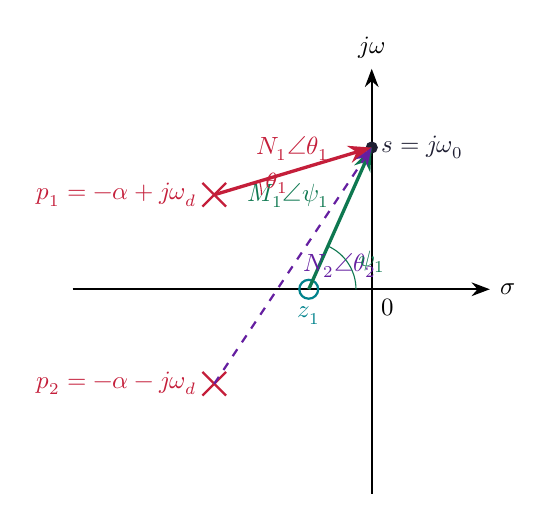
\begin{tikzpicture}[scale=1.0, every node/.style={font=\small}]
  % Axes
  \draw[-Stealth, thick] (-3.8,0) -- (1.5,0) node[right] {$\sigma$};
  \draw[-Stealth, thick] (0,-2.6) -- (0,2.8) node[above] {$j\omega$};

  % Origin
  \node[below right] at (0,0) {$0$};

  % Poles and Zeros
  \coordinate (P1) at (-2.0, 1.2);
  \coordinate (P2) at (-2.0, -1.2);
  \coordinate (Z1) at (-0.8, 0);
  \coordinate (JW) at (0, 1.8);

  % Draw Poles (X) and Zeros (O)
  \draw[thick, color=myred] ($(P1)+(-0.15,-0.15)$) -- ($(P1)+(0.15,0.15)$);
  \draw[thick, color=myred] ($(P1)+(-0.15,0.15)$) -- ($(P1)+(0.15,-0.15)$);
  \node[left=0.1cm of P1, color=myred] {$p_1 = -\alpha + j\omega_d$};

  \draw[thick, color=myred] ($(P2)+(-0.15,-0.15)$) -- ($(P2)+(0.15,0.15)$);
  \draw[thick, color=myred] ($(P2)+(-0.15,0.15)$) -- ($(P2)+(0.15,-0.15)$);
  \node[left=0.1cm of P2, color=myred] {$p_2 = -\alpha - j\omega_d$};

  \draw[thick, color=myteal] (Z1) circle (0.12);
  \node[below=0.1cm of Z1, color=myteal] {$z_1$};

  % Evaluation point on jw axis
  \filldraw[color=mydark] (JW) circle (0.07) node[right] {$s = j\omega_0$};

  % Vectors from pole/zero to jw point
  \draw[-Stealth, very thick, color=mygreen] (Z1) -- (JW) node[midway, above left] {$M_1 \angle \psi_1$};
  \draw[-Stealth, very thick, color=myred] (P1) -- (JW) node[midway, above] {$N_1 \angle \theta_1$};
  \draw[-Stealth, thick, dashed, color=mypurple] (P2) -- (JW) node[midway, right] {$N_2 \angle \theta_2$};

  % Angle arcs
  \draw[thin, color=mygreen] ($(Z1)+(0.6,0)$) arc (0:66:0.6);
  \node[color=mygreen, font=\footnotesize] at ($(Z1)+(0.8,0.35)$) {$\psi_1$};

  \draw[thin, color=myred] ($(P1)+(0.6,0)$) arc (0:17:0.6);
  \node[color=myred, font=\footnotesize] at ($(P1)+(0.8,0.15)$) {$\theta_1$};
\end{tikzpicture}
\end{center}
\end{tcolorbox}

% ===============================================================================
% SECTION 4: CONVOLUTION THEOREM IN ELECTRICAL CIRCUITS
% ===============================================================================
\section{The Convolution Theorem in Electrical Networks}

The convolution theorem establishes the fundamental mathematical bridge between time-domain input-output relationships and $s$-domain transfer function multiplication.

\subsection{Mathematical Definition and Circuit Interpretation}

\begin{tcolorbox}[defbox, title={\textbf{Time Convolution Theorem}}]
Let $h(t)$ be the \textbf{impulse response} of a relaxed LTI network (the response when excited by $x(t) = \delta(t)$). The zero-state response $y(t)$ to an arbitrary continuous excitation $x(t)$ applied at $t=0$ is given by the convolution integral:
\begin{equation}
  y(t) = x(t) * h(t) = \int_{0^-}^t x(\tau)\,h(t - \tau)\,d\tau = \int_{0^-}^t h(\tau)\,x(t - \tau)\,d\tau
\end{equation}
In the transformed frequency domain:
\begin{equation}
  \mathcal{L}\{x(t) * h(t)\} = X(s) \cdot H(s) \iff Y(s) = H(s) X(s)
\end{equation}
where $H(s) = \mathcal{L}\{h(t)\}$ is the transfer function of the network.
\end{tcolorbox}

\begin{tcolorbox}[formulabox, title={\textbf{Relation Between Impulse Response and Step Response}}]
If $s(t)$ represents the unit step response ($x(t) = u(t)$) of a linear network:
\begin{equation}
  s(t) = u(t) * h(t) = \int_{0^-}^t h(\tau)\,d\tau \iff h(t) = \frac{ds(t)}{dt}
\end{equation}
The unit impulse response is the exact time derivative of the unit step response.
\end{tcolorbox}

% ===============================================================================
% SECTION 5: TWO-PORT NETWORK PARAMETERS AND INTERCONNECTIONS
% ===============================================================================
\section{Two-Port Network Parameters and Interconnections}

A two-port network is a four-terminal electrical network having two distinct access ports: Port 1 (input port, terminals $1-1'$) and Port 2 (output port, terminals $2-2'$). Standard sign convention assumes terminal currents $I_1$ and $I_2$ enter the positive terminal of their respective ports.

\begin{tcolorbox}[tikzbox, title={\textbf{TikZ Schematic: Standard Terminal Variable Convention for a Two-Port Network}}]
\begin{center}
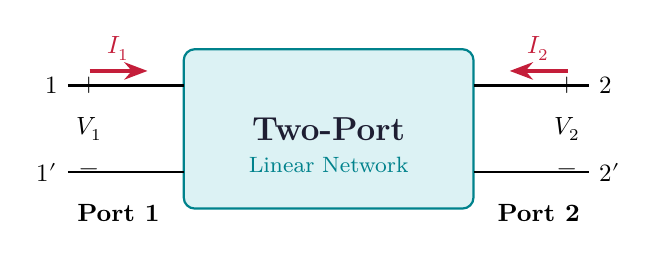
\begin{tikzpicture}[scale=0.92, every node/.style={font=\small}]
  % Two-port box
  \draw[thick, fill=hdrteal, draw=myteal, rounded corners=4pt] (2,0) rectangle (6,2.2);
  \node[font=\large\bfseries\color{mydark}] at (4,1.1) {Two-Port};
  \node[font=\footnotesize\color{myteal}] at (4,0.6) {Linear Network};

  % Port 1
  \draw[thick] (0.4,1.7) node[left] {$1$} -- (2,1.7);
  \draw[thick] (0.4,0.5) node[left] {$1'$} -- (2,0.5);
  \draw[-Stealth, very thick, color=myred] (0.7,1.9) -- (1.5,1.9) node[midway, above] {$I_1$};
  \node at (0.7, 1.7) {$+$};
  \node at (0.7, 0.5) {$-$};
  \node at (0.7, 1.1) {$V_1$};
  \node[below=0.1cm] at (1.1,0.3) {\textbf{Port 1}};

  % Port 2
  \draw[thick] (6,1.7) -- (7.6,1.7) node[right] {$2$};
  \draw[thick] (6,0.5) -- (7.6,0.5) node[right] {$2'$};
  \draw[-Stealth, very thick, color=myred] (7.3,1.9) -- (6.5,1.9) node[midway, above] {$I_2$};
  \node at (7.3, 1.7) {$+$};
  \node at (7.3, 0.5) {$-$};
  \node at (7.3, 1.1) {$V_2$};
  \node[below=0.1cm] at (6.9,0.3) {\textbf{Port 2}};
\end{tikzpicture}
\end{center}
\end{tcolorbox}

\subsection{The Six Fundamental Two-Port Parameter Sets}

\begin{tcolorbox}[defbox, title={\textbf{Definitions and Equations of Two-Port Parameter Sets}}]
\begin{enumerate}[leftmargin=*, itemsep=4pt]
  \item \textbf{Impedance ($Z$) Parameters (Open-Circuit Parameters):}
  \begin{equation}
    \begin{bmatrix} V_1 \\ V_2 \end{bmatrix} = \begin{bmatrix} z_{11} & z_{12} \\ z_{21} & z_{22} \end{bmatrix} \begin{bmatrix} I_1 \\ I_2 \end{bmatrix} \implies \begin{aligned} V_1 &= z_{11} I_1 + z_{12} I_2 \\ V_2 &= z_{21} I_1 + z_{22} I_2 \end{aligned}
  \end{equation}
  $z_{11} = \left.\frac{V_1}{I_1}\right|_{I_2=0}$ (input impedance), $z_{12} = \left.\frac{V_1}{I_2}\right|_{I_1=0}$ (reverse transfer impedance),\\
  $z_{21} = \left.\frac{V_2}{I_1}\right|_{I_2=0}$ (forward transfer impedance), $z_{22} = \left.\frac{V_2}{I_2}\right|_{I_1=0}$ (output impedance).

  \item \textbf{Admittance ($Y$) Parameters (Short-Circuit Parameters):}
  \begin{equation}
    \begin{bmatrix} I_1 \\ I_2 \end{bmatrix} = \begin{bmatrix} y_{11} & y_{12} \\ y_{21} & y_{22} \end{bmatrix} \begin{bmatrix} V_1 \\ V_2 \end{bmatrix} \implies \begin{aligned} I_1 &= y_{11} V_1 + y_{12} V_2 \\ I_2 &= y_{21} V_1 + y_{22} V_2 \end{aligned}
  \end{equation}
  $[Y] = [Z]^{-1} \implies y_{11} = \frac{z_{22}}{\Delta z}, \quad y_{12} = -\frac{z_{12}}{\Delta z}, \quad y_{21} = -\frac{z_{21}}{\Delta z}, \quad y_{22} = \frac{z_{11}}{\Delta z}$.

  \item \textbf{Transmission ($ABCD$) Parameters (Cascade / Chain Parameters):}
  Relates input terminal variables to output terminal variables under reverse current load convention:
  \begin{equation}
    \begin{bmatrix} V_1 \\ I_1 \end{bmatrix} = \begin{bmatrix} A & B \\ C & D \end{bmatrix} \begin{bmatrix} V_2 \\ -I_2 \end{bmatrix} \implies \begin{aligned} V_1 &= A V_2 - B I_2 \\ I_1 &= C V_2 - D I_2 \end{aligned}
  \end{equation}
  $A = \left.\frac{V_1}{V_2}\right|_{I_2=0}$ (reverse voltage ratio), $B = \left.\frac{V_1}{-I_2}\right|_{V_2=0}$ (transfer impedance),\\
  $C = \left.\frac{I_1}{V_2}\right|_{I_2=0}$ (transfer admittance), $D = \left.\frac{I_1}{-I_2}\right|_{V_2=0}$ (reverse current ratio).

  \item \textbf{Hybrid ($h$) Parameters:}
  Used extensively in small-signal bipolar transistor modeling:
  \begin{equation}
    \begin{bmatrix} V_1 \\ I_2 \end{bmatrix} = \begin{bmatrix} h_{11} & h_{12} \\ h_{21} & h_{22} \end{bmatrix} \begin{bmatrix} I_1 \\ V_2 \end{bmatrix} \implies \begin{aligned} V_1 &= h_{11} I_1 + h_{12} V_2 \\ I_2 &= h_{21} I_1 + h_{22} V_2 \end{aligned}
  \end{equation}

  \item \textbf{Inverse Hybrid ($g$) Parameters:}
  Used in field-effect transistor modeling:
  \begin{equation}
    \begin{bmatrix} I_1 \\ V_2 \end{bmatrix} = \begin{bmatrix} g_{11} & g_{12} \\ g_{21} & g_{22} \end{bmatrix} \begin{bmatrix} V_1 \\ I_2 \end{bmatrix} \implies \begin{aligned} I_1 &= g_{11} V_1 + g_{12} I_2 \\ V_2 &= g_{21} V_1 + g_{22} I_2 \end{aligned}
  \end{equation}
\end{enumerate}
\end{tcolorbox}

\subsection{Reciprocity and Symmetry Conditions}

\par\vspace{6pt}\noindent
\begingroup
\setlength{\tabcolsep}{5pt}
\setlength{\extrarowheight}{3pt}
\renewcommand{\arraystretch}{1.38}
\begin{tabularx}{\linewidth}{|B{3.5cm}|B{4.0cm}|Y|}
\hline
\multicolumn{1}{|c|}{\textbf{Parameter Set}} & \multicolumn{1}{c|}{\textbf{Reciprocity Condition}} & \multicolumn{1}{c|}{\textbf{Symmetry Condition}} \\
\hline
Impedance ($Z$) & $z_{12} = z_{21}$ & $z_{11} = z_{22}$ \\
\hline
Admittance ($Y$) & $y_{12} = y_{21}$ & $y_{11} = y_{22}$ \\
\hline
Transmission ($ABCD$) & $AD - BC = 1$ & $A = D$ \\
\hline
Hybrid ($h$) & $h_{12} = -h_{21}$ & $\Delta h = h_{11} h_{22} - h_{12} h_{21} = 1$ \\
\hline
Inverse Hybrid ($g$) & $g_{12} = -g_{21}$ & $\Delta g = g_{11} g_{22} - g_{12} g_{21} = 1$ \\
\hline
\end{tabularx}
\endgroup
\vspace{12pt}

\subsection{Interconnections of Two-Port Networks}

When two-port networks $N_A$ and $N_B$ are interconnected, their overall parameter matrices combine algebraically:

\begin{tcolorbox}[defbox, title={\textbf{Combination Rules for Interconnected Two-Ports}}]
\begin{enumerate}[leftmargin=*]
  \item \textbf{Series-Series Connection:} Input ports connected in series, output ports in series:
  \begin{equation}
    [Z] = [Z_A] + [Z_B]
  \end{equation}
  \item \textbf{Parallel-Parallel Connection:} Input ports in parallel, output ports in parallel:
  \begin{equation}
    [Y] = [Y_A] + [Y_B]
  \end{equation}
  \item \textbf{Cascade (Tandem) Connection:} Output of $N_A$ connected to input of $N_B$:
  \begin{equation}
    [T] = [T_A] \times [T_B] = \begin{bmatrix} A_A & B_A \\ C_A & D_A \end{bmatrix} \begin{bmatrix} A_B & B_B \\ C_B & D_B \end{bmatrix}
  \end{equation}
  \item \textbf{Series-Parallel Connection:} Input ports in series, output ports in parallel:
  \begin{equation}
    [h] = [h_A] + [h_B]
  \end{equation}
\end{enumerate}
\textbf{Brune's Test for Validity:} When combining two-port networks in series or parallel, circulating loop currents between the two networks can violate the fundamental port condition ($i_{\text{in}} = i_{\text{return}}$). Brune's test confirms validity: if the terminal voltage across the interconnection points is zero before connection, the matrices can be added directly without ideal isolation transformers.
\end{tcolorbox}

% ===============================================================================
% SECTION 6: SERIES AND PARALLEL RESONANCE
% ===============================================================================
\section{Behaviors of Series and Parallel Resonant Circuits}

Resonance is a phenomenon in reactive circuits where inductive and capacitive reactances cancel each other out at a specific frequency, causing the total input impedance to become purely real and the circuit power factor to equal unity ($\cos\phi = 1$).

\subsection{Series Resonance}

Consider an RLC branch connected in series across an AC source $\mathbf{V}$. The total complex impedance is:
\begin{equation}
  \mathbf{Z}(j\omega) = R + j\left(\omega L - \frac{1}{\omega C}\right)
\end{equation}

\begin{tcolorbox}[formulabox, title={\textbf{Series Resonance Equations}}]
\begin{enumerate}[leftmargin=*]
  \item \textbf{Resonance Condition:} Net reactance is identically zero:
  \begin{equation}
    X_L = X_C \implies \omega_0 L = \frac{1}{\omega_0 C} \implies \omega_0 = \frac{1}{\sqrt{LC}} \text{ rad/s}, \quad f_0 = \frac{1}{2\pi\sqrt{LC}} \text{ Hz}
  \end{equation}
  \item \textbf{Impedance at Resonance:} Minimum and purely resistive:
  \begin{equation}
    \mathbf{Z}(j\omega_0) = Z_{\min} = R \implies \mathbf{I}_0 = \frac{\mathbf{V}}{R} \quad (\text{Maximum Current})
  \end{equation}
  \item \textbf{Quality Factor ($Q$):} Defined as $2\pi \times \frac{\text{Maximum Energy Stored}}{\text{Energy Dissipated per Cycle}}$:
  \begin{equation}
    Q_0 = \frac{\omega_0 L}{R} = \frac{1}{\omega_0 C R} = \frac{1}{R}\sqrt{\frac{L}{C}}
  \end{equation}
  \item \textbf{Voltage Magnification:} Reactive voltages across $L$ and $C$ can far exceed source voltage:
  \begin{equation}
    V_L(j\omega_0) = V_C(j\omega_0) = Q_0 \cdot V
  \end{equation}
  \item \textbf{Half-Power Frequencies and Bandwidth ($BW$):}
  The frequencies $\omega_1$ (lower) and $\omega_2$ (upper) where current magnitude drops to $I_0/\sqrt{2}$ ($70.7\%$) and dissipated active power drops to $P_{\max}/2$:
  \begin{equation}
    \omega_{1,2} = \mp \frac{R}{2L} + \sqrt{\left(\frac{R}{2L}\right)^2 + \frac{1}{LC}} \implies BW = \Delta\omega = \omega_2 - \omega_1 = \frac{R}{L} = \frac{\omega_0}{Q_0}
  \end{equation}
  Geometric center frequency relation: $\omega_0 = \sqrt{\omega_1 \omega_2}$. For high-$Q$ circuits ($Q \ge 10$), arithmetic symmetry holds: $\omega_1 \approx \omega_0 - \frac{BW}{2}, \quad \omega_2 \approx \omega_0 + \frac{BW}{2}$.
\end{enumerate}
\end{tcolorbox}

\subsection{Parallel Resonance (Practical Tank Circuit)}

A practical inductor possesses winding resistance $R_L$. The practical parallel tank consists of a coil ($R_L$ in series with $L$) connected in parallel with an ideal capacitor $C$.
\begin{equation}
  \mathbf{Y} = \frac{1}{R_L + j\omega L} + j\omega C = \frac{R_L - j\omega L}{R_L^2 + \omega^2 L^2} + j\omega C = \frac{R_L}{R_L^2 + \omega^2 L^2} + j\left(\omega C - \frac{\omega L}{R_L^2 + \omega^2 L^2}\right)
\end{equation}

\begin{tcolorbox}[defbox, title={\textbf{Practical Tank Circuit Resonance Conditions}}]
\begin{enumerate}[leftmargin=*]
  \item \textbf{Unity Power Factor Resonant Frequency $\omega_r$:} Setting net susceptance to zero:
  \begin{equation}
    \omega_r C = \frac{\omega_r L}{R_L^2 + \omega_r^2 L^2} \implies \omega_r = \sqrt{\frac{1}{LC} - \frac{R_L^2}{L^2}} = \omega_0\sqrt{1 - \frac{R_L^2 C}{L}}
  \end{equation}
  Physical condition for parallel resonance to occur: $\dfrac{L}{C} > R_L^2$.
  \item \textbf{Dynamic Impedance ($Z_d$):} At resonance, the circuit exhibits \textbf{maximum impedance} (anti-resonance):
  \begin{equation}
    Z_d = \frac{1}{Y_{\min}} = \frac{R_L^2 + \omega_r^2 L^2}{R_L} = \frac{L}{C R_L} \quad (\Omega)
  \end{equation}
  Total line current is minimum: $I_{\min} = \frac{V}{Z_d} = \frac{V C R_L}{L}$.
  \item \textbf{Current Magnification:} Circulating loop current between coil and capacitor is $Q$ times line current:
  \begin{equation}
    I_{\text{circ}} \approx Q \cdot I_{\text{line}}, \quad \text{where } Q = \frac{\omega_r L}{R_L}
  \end{equation}
\end{enumerate}
\end{tcolorbox}

% ===============================================================================
% SECTION 7: INTRODUCTION TO PASSIVE FILTERS
% ===============================================================================
\section{Introduction to Passive Electric Filters}

An electric filter is a frequency-selective two-port network designed to transmit signals within specified frequency bands (\textbf{pass bands}) with minimal attenuation, while significantly attenuating signals outside those bands (\textbf{attenuation / stop bands}).

\subsection{Propagation Characteristics and Cut-Off Frequency}

For a symmetrical reactive network terminated in its characteristic impedance $Z_0$:
\begin{equation}
  \frac{\mathbf{V}_1}{\mathbf{V}_2} = \frac{\mathbf{I}_1}{\mathbf{I}_2} = e^\gamma = e^{\alpha + j\beta} \implies \gamma = \alpha + j\beta
\end{equation}
where $\gamma$ is the complex propagation constant, $\alpha$ is the attenuation constant (in Nepers), and $\beta$ is the phase shift constant (in radians).
\begin{itemize}[leftmargin=*]
  \item \textbf{Pass Band:} $\alpha = 0$, signals pass with zero attenuation ($|\mathbf{V}_2/\mathbf{V}_1| = 1$), experiencing only a phase delay $\beta$.
  \item \textbf{Stop Band:} $\alpha > 0$, signal amplitude decays exponentially.
  \item \textbf{Cut-Off Frequency ($f_c$):} The boundary frequency demarcating the pass band from the stop band, defined where $\alpha = 0$ begins to increase.
\end{itemize}

\subsection{Constant-$k$ Prototype Filter Sections}

A symmetrical ladder network has series impedance $Z_1$ and shunt impedance $Z_2$. It is termed a \textbf{constant-$k$ filter} if:
\begin{equation}
  Z_1 \cdot Z_2 = k^2 = R_0^2 \quad (\text{independent of frequency})
\end{equation}
where $R_0 = \sqrt{L/C}$ is the nominal design characteristic resistance.

\par\vspace{6pt}\noindent
\begingroup
\setlength{\tabcolsep}{4.0pt}
\setlength{\extrarowheight}{2.5pt}
\renewcommand{\arraystretch}{1.25}
\begin{tabularx}{\linewidth}{|B{2.5cm}|B{3.0cm}|B{3.0cm}|Y|}
\hline
\textbf{Filter Type} & \textbf{Series Arm $Z_1$} & \textbf{Shunt Arm $Z_2$} & \textbf{Cut-off \& Design Formulas} \\
\hline
Low-Pass (LPF) & Inductor $L$ ($j\omega L$) & Capacitor $C$ ($\frac{1}{j\omega C}$) & $f_c = \frac{1}{\pi\sqrt{LC}}$,\\[2pt]$L = \frac{R_0}{\pi f_c}, \quad C = \frac{1}{\pi f_c R_0}$ \\
\hline
High-Pass (HPF) & Capacitor $C$ ($\frac{1}{j\omega C}$) & Inductor $L$ ($j\omega L$) & $f_c = \frac{1}{4\pi\sqrt{LC}}$,\\[2pt]$L = \frac{R_0}{4\pi f_c}, \quad C = \frac{1}{4\pi f_c R_0}$ \\
\hline
Band-Pass (BPF) & Series resonant ($L_1, C_1$) & Parallel resonant ($L_2, C_2$) & $f_0 = \sqrt{f_1 f_2}, \quad BW = f_2 - f_1$ \\
\hline
Band-Reject (BRF) & Parallel resonant ($L_1, C_1$) & Series resonant ($L_2, C_2$) & Stops band between $f_1$ and $f_2$; passes DC and high AC. \\
\hline
\end{tabularx}
\endgroup
\vspace{12pt}

\begin{tcolorbox}[masonbox, title={\textbf{Limitations of Constant-$k$ Filters and Evolution to $m$-Derived Filters}}]
\begin{enumerate}[leftmargin=*]
  \item \textbf{Gradual Attenuation Rise:} The attenuation $\alpha$ of a constant-$k$ filter rises slowly beyond the cut-off frequency $f_c$.
  \item \textbf{Mismatched Terminal Impedance:} The characteristic impedance $Z_{0T}(f)$ or $Z_{0\pi}(f)$ varies widely across the pass band and drops to zero or infinity at $f_c$, creating severe reflection losses when terminated in a fixed resistance $R_0$.
  \item \textbf{$m$-Derived Filter Fix:} By incorporating a tuning parameter $m = \sqrt{1 - (f_c/f_\infty)^2}$ ($0 < m \le 1$), an infinite attenuation notch ($f_\infty$) is introduced near the cut-off frequency, producing an extraordinarily sharp transition and a nearly constant characteristic impedance over $85\%$ of the pass band.
\end{enumerate}
\end{tcolorbox}

\newpage
% ===============================================================================
% MANDATORY QUICK REVISION PAGE
% ===============================================================================
\begin{center}
  {\large\bfseries\color{myred} Quick Revision --- Module 4}\\[2pt]
  {\small\color{mydark} Network Functions, Two-Port Networks, Resonance and Filters $|$ EC304}
\end{center}
\noindent{\color{myred}\rule{\linewidth}{1.0pt}}
\vspace{2pt}

\begin{tcolorbox}[formulabox, top=5pt, bottom=5pt, title={\textbf{Key Formulas and Network Relations at a Glance}}]
\renewcommand{\arraystretch}{1.20}
\begin{tabularx}{\linewidth}{B{5.0cm} X}
Complex Frequency & $s = \sigma + j\omega \quad (\sigma: \text{Np/s}, \; \omega: \text{rad/s})$ \\[2pt]
Magnitude from Pole-Zero & $|H(j\omega)| = |K| \frac{\prod |j\omega - z_i|}{\prod |j\omega - p_k|} = |K| \frac{\text{Distance product from zeros}}{\text{Distance product from poles}}$ \\[2pt]
Phase from Pole-Zero & $\angle H(j\omega) = \sum \angle(j\omega - z_i) - \sum \angle(j\omega - p_k)$ \\[2pt]
$Z$ to $Y$ Matrix Inverse & $[Y] = [Z]^{-1}, \quad y_{11} = \frac{z_{22}}{\Delta z}, \; y_{12} = -\frac{z_{12}}{\Delta z}, \; y_{22} = \frac{z_{11}}{\Delta z}$ \\[2pt]
$ABCD$ Transmission Cascade & $[T_{\text{total}}] = [T_A] \times [T_B], \quad AD - BC = 1 \text{ (Reciprocity)}$ \\[2pt]
Series Resonance & $\omega_0 = \frac{1}{\sqrt{LC}}, \quad Z_{\min} = R, \quad Q = \frac{\omega_0 L}{R} = \frac{1}{R}\sqrt{\frac{L}{C}}$ \\[2pt]
Bandwidth \& Selectivity & $BW = \omega_2 - \omega_1 = \frac{R}{L} = \frac{\omega_0}{Q}, \quad \omega_0 = \sqrt{\omega_1 \omega_2}$ \\[2pt]
Parallel Dynamic Impedance & $\omega_r = \sqrt{\frac{1}{LC} - \frac{R_L^2}{L^2}}, \quad Z_d = \frac{L}{C R_L} \quad (\text{Max Impedance})$ \\[2pt]
Constant-$k$ LPF Cut-off & $f_c = \frac{1}{\pi\sqrt{LC}}, \quad L = \frac{R_0}{\pi f_c}, \quad C = \frac{1}{\pi f_c R_0}$ \\[2pt]
\end{tabularx}
\end{tcolorbox}

\begin{tcolorbox}[defbox, top=5pt, bottom=5pt, title={\textbf{One-Line Definitions}}]
\begin{itemize}[leftmargin=*, itemsep=1.0pt, topsep=0pt]
  \item \textbf{Complex Frequency ($s$):} Variable $s = \sigma + j\omega$ combining exponential damping rate and oscillation frequency.
  \item \textbf{Driving-Point Immittance:} The input impedance or admittance measured across a single terminal pair with internal relaxed state.
  \item \textbf{Transfer Function:} Ratio of response transform at one port to excitation transform at another port under zero initial states.
  \item \textbf{Hurwitz Polynomial:} A polynomial having all its roots located strictly in the closed left half of the complex $s$-plane.
  \item \textbf{Positive Real (PR) Function:} A rational function $Z(s)$ whose real part is non-negative whenever the real part of $s$ is non-negative.
  \item \textbf{Impulse Response $h(t)$:} Time-domain output of an initially relaxed network when driven by an ideal Dirac delta excitation.
  \item \textbf{Quality Factor ($Q$):} Dimensionless figure of merit measuring energy storage efficiency relative to per-cycle dissipation.
  \item \textbf{Anti-Resonance:} Parallel resonance state exhibiting maximum terminal impedance and minimum source line current.
  \item \textbf{Cut-Off Frequency ($f_c$):} Frequency demarcating pass band ($\alpha = 0$) from stop band ($\alpha > 0$) in a filter network.
  \item \textbf{$m$-Derived Filter:} Modified ladder section with a resonance trap providing sharp attenuation notch and flat $Z_0$.
\end{itemize}
\end{tcolorbox}

\begin{tcolorbox}[exambox, title={\textbf{Frequently Asked / Viva Questions}}]
\begin{enumerate}[topsep=0pt, label=\textbf{Q\arabic*.}, itemsep=2.2pt]
  \item \Q{What are the necessary conditions for a rational function to be a Positive Real (PR) function?}
  $Z(s)$ must have real coefficients; all poles and zeros must lie in the left half $s$-plane; $j\omega$-axis poles must be simple with real, positive residues; and degrees of $N(s)$ and $D(s)$ can differ at most by $1$.

  \item \Q{Why must poles and zeros alternate on the imaginary axis for an LC driving-point immittance?}
  By Foster's Reactance Theorem, $\frac{dX(\omega)}{d\omega} > 0$ strictly holds for lossless LC networks. Reactance increases monotonically with frequency, forcing every zero ($X=0$) to be succeeded by a pole ($X \to \infty$).

  \item \Q{State the condition for reciprocity and symmetry in terms of $ABCD$ parameters.}
  Reciprocity holds if the transmission determinant is unity: $AD - BC = 1$. The network is symmetrical (electrically identical when ports are interchanged) if $A = D$.

  \item \Q{Explain why series resonance gives 'voltage magnification' and parallel resonance 'current magnification'.}
  At series resonance, current is maximum, producing reactive voltages across $L$ and $C$ equal to $Q$ times input voltage ($V_L = V_C = Q V$). At parallel resonance, circulating current between $L$ and $C$ equals $Q$ times line current ($I_{\text{circ}} = Q I$).

  \item \Q{What is Brune's Test, and why is it conducted before interconnecting two-port networks?}
  Brune's test verifies whether interconnecting two-ports creates circulating loop currents that violate the port condition ($I_{\text{in}} = I_{\text{out}}$). If open-circuit ground potential is non-zero, an ideal $1:1$ isolation transformer is required.

  \item \Q{How does winding resistance $R_L$ affect practical parallel tank resonant frequency?}
  Winding resistance lowers resonant frequency below the ideal value: $\omega_r = \sqrt{\frac{1}{LC} - \frac{R_L^2}{L^2}} = \omega_0\sqrt{1 - \frac{R_L^2 C}{L}}$. If $R_L \ge \sqrt{L/C}$, resonance cannot occur.

  \item \Q{State the relationship between resonant frequency $\omega_0$ and half-power frequencies in series resonance.}
  $\omega_0$ is the exact geometric mean of half-power frequencies: $\omega_0 = \sqrt{\omega_1 \omega_2}$. For high-$Q$ circuits ($Q \ge 10$), it is also approximately their arithmetic mean: $\omega_0 \approx (\omega_1 + \omega_2)/2$.

  \item \Q{Why does a constant-$k$ filter have undesirable impedance characteristics in its pass band?}
  Its characteristic impedance $Z_{0T}(f) = R_0\sqrt{1 - (f/f_c)^2}$ drops to zero at $f_c$, while $Z_{0\pi}(f)$ approaches infinity. This impedance mismatch causes large reflection losses near cut-off when terminated in $R_0$.

  \item \Q{What is the physical meaning of poles in a network transfer function?}
  Poles represent the complex natural frequencies (modes) of the system. The real part dictates exponential decay or growth rate, while the imaginary part specifies unforced transient oscillation frequency.

  \item \Q{State the relationship between convolution in time and transfer function in frequency domain.}
  In the time domain, response is the convolution of input with the impulse response: $y(t) = x(t) * h(t)$. In the $s$-domain, this integral simplifies into algebraic multiplication: $Y(s) = H(s) \cdot X(s)$.
\end{enumerate}
\end{tcolorbox}

\begin{tcolorbox}[tikzbox, top=4pt, bottom=4pt, title={\textbf{Summary Matrix: Comprehensive Comparison of Two-Port Parameters and Resonant Circuits}}]
\par\vspace{2pt}\noindent
\begingroup
\setlength{\tabcolsep}{3.5pt}
\setlength{\extrarowheight}{1.5pt}
\renewcommand{\arraystretch}{1.18}
\begin{tabularx}{\linewidth}{|B{2.5cm}|B{3.8cm}|B{2.7cm}|Y|}
\hline
\textbf{Parameter / Circuit} & \textbf{Key Governing Relations} & \textbf{Reciprocity / Symmetry} & \textbf{Circuit Application} \\
\hline
$Z$-Parameters & $V_1 = z_{11} I_1 + z_{12} I_2$\\[1pt]$V_2 = z_{21} I_1 + z_{22} I_2$ & $z_{12} = z_{21}$\\[1pt]$z_{11} = z_{22}$ & Open-circuit test; series-series connections. \\
\hline
$Y$-Parameters & $I_1 = y_{11} V_1 + y_{12} V_2$\\[1pt]$I_2 = y_{21} V_1 + y_{22} V_2$ & $y_{12} = y_{21}$\\[1pt]$y_{11} = y_{22}$ & Short-circuit test; parallel-parallel connections. \\
\hline
$ABCD$-Parameters & $V_1 = A V_2 - B I_2$\\[1pt]$I_1 = C V_2 - D I_2$ & $AD - BC = 1$\\[1pt]$A = D$ & Transmission lines; cascaded stage networks. \\
\hline
$h$-Parameters & $V_1 = h_{11} I_1 + h_{12} V_2$\\[1pt]$I_2 = h_{21} I_1 + h_{22} V_2$ & $h_{12} = -h_{21}$\\[1pt]$\Delta h = 1$ & Transistor hybrid small-signal equivalent circuits. \\
\hline
Series Resonant Circuit & $\omega_0 = 1/\sqrt{LC}, \; Z_{\min} = R$\\[1pt]$Q = \omega_0 L / R$ & $V_L = V_C = Q V$\\[1pt](Resonance) & Wave traps; radio tuners; voltage magnification. \\
\hline
Parallel Resonant Tank & $\omega_r = \sqrt{\frac{1}{LC} - \frac{R_L^2}{L^2}}$\\[1pt]$Z_d = \frac{L}{C R_L}$ (Max $Z$) & $I_{\text{circ}} = Q I_{\text{line}}$\\[1pt](Anti-resonance) & RF tank circuits; oscillators; high-impedance loads. \\
\hline
\end{tabularx}
\endgroup
\end{tcolorbox}

\end{document}
